% !TEX root = ../main.tex

% 中英标题:\chapter{中文标题}[英文标题]
\chapter{过驱动多旋翼飞行器的结构设计与动力学分析}\label{chap:structure_and_dynamics}

\section{引言}\label{sec:intro_2}
过驱动多旋翼飞行器的结构和动力学模型相较传统欠驱动多旋翼飞行器而言有较大不同,为了科学地为其设计运动规划算法,有必要对其结构和动力学模型进行分析。
本章~\ref{sec:structure_design}节对本课题所使用的过驱动多旋翼平台OmniHex的设计进行简要介绍;
\ref{sec:dynamic_analysis}节建立OmniHex的动力学模型,并分析其微分平坦性质。
% \ref{sec:control_policy}节对OmniHex的控制策略作简要介绍。

\section{过驱动多旋翼飞行器的设计}\label{sec:structure_design}
成功搭建一台过驱动飞行器的要点在于为其设计合理的机械与电子系统,本节就从机械结构设计与航电系统设计两方面对本课题所搭建的OmniHex飞行器(\figref{fig:real_overview})进行介绍。
\begin{figure}[ht]
    \centering
    \includegraphics[width = 0.65\textwidth]{real_overview.jpg}
    \caption{OmniHex飞行器实物示意图}
    \label{fig:real_overview}
\end{figure}
\subsection{机械结构设计}\label{subsec:mechanical_structure_design}
OmniHex采用类似Voliro的可倾转旋翼构型,\figref{fig:omni_hex_structure}展示了其机械结构外观,并对重要部件做出了标注。
OmniHex的每个旋翼除了可以绕电机轴进行旋转以提供推力外,其指向还可以在舵机的驱动下随着机臂绕机臂轴线旋转,
如\figref{fig:structure_detail_1}和\figref{fig:structure_detail_2}所示,
驱动旋翼的无刷电机与机臂固连在一起,所以旋翼与其所在的机臂是同时倾转的;
舵机安装于组成机身的两块中心板之间,且个舵机都位于其所驱动的机臂根部,二者之间由一个舵机-机臂连接件进行桥接,
舵机的舵盘旋转时,将动力传递给连接件,连接件再将动力经由固定用的螺栓传递给机臂。
为防止机臂倾转造成线缆缠绕,需要连接无刷电机与电子调速器(固定于机身)的三相线在机臂位于倾转零点时预留有一定长度。
\begin{figure}[!ht]
    \setlength{\subfigcapskip}{-1bp}
    \centering
    \begin{minipage}{\textwidth}
    \centering
    \subfigure{\label{fig:structure_overview}}\addtocounter{subfigure}{-2}
    \subfigure{\subfigure[整体结构概览]{\includegraphics[width=0.45\textwidth]{structure_overview.png}}}
    \hspace{0.2em}
    \subfigure{\label{fig:structure_detail_1}}\addtocounter{subfigure}{-2}
    \subfigure{\subfigure[倾转旋翼单元结构图1]{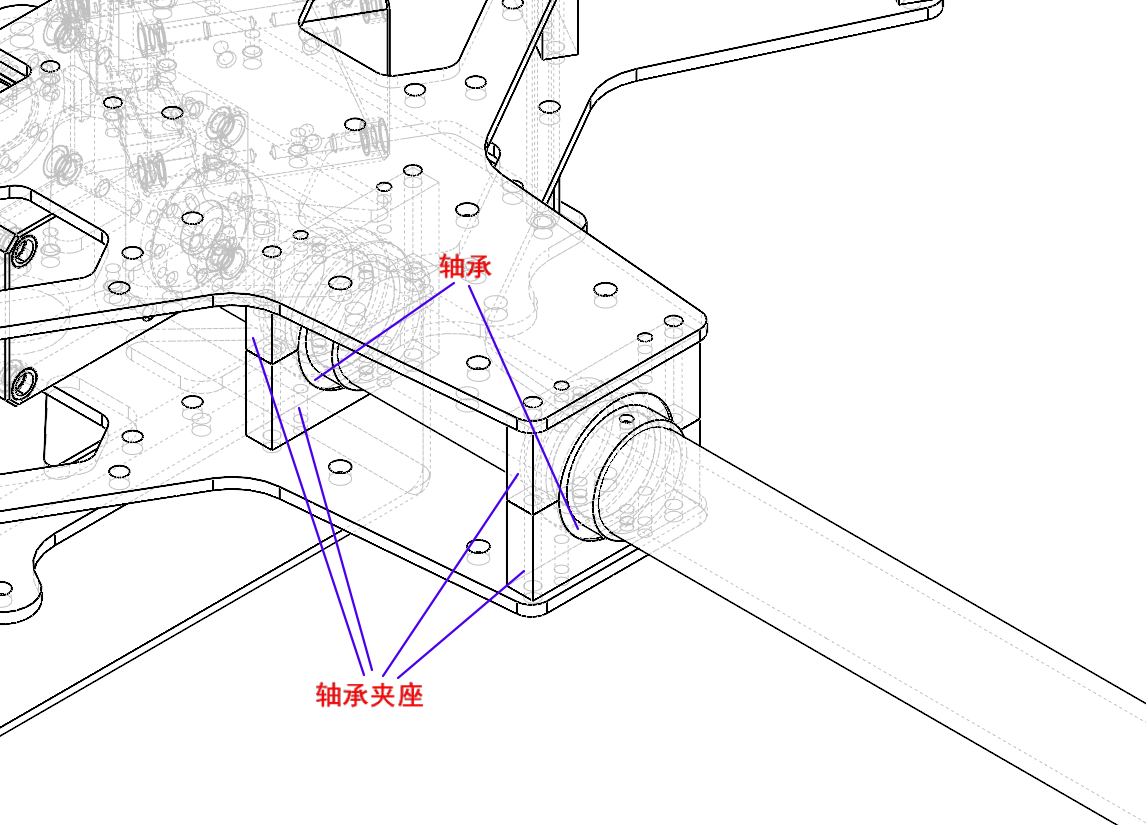
\includegraphics[width=0.45\textwidth]{structure_detail_1.png}}}

	\subfigure{\label{fig:structure_detail_2}}\addtocounter{subfigure}{-2}
    \subfigure{\subfigure[倾转旋翼单元结构图2]{\includegraphics[width=0.9\textwidth]{structure_detail_2.png}}}
    \end{minipage}
    \caption{OmniHex机械结构示意图\label{fig:omni_hex_structure}}
\end{figure}

每一个旋翼-无刷电机组合,与其所在的机臂及相应舵机一起组成了一个倾转旋翼单元,为飞行器带来了两个机械自由度,
OmniHex上安装了6个独立的倾转旋翼单元,故拥有12个机械自由度。
每个倾转旋翼单元不仅在舵机处与机身相连,为了防止组成机臂的柔软碳管发生弯曲形变,还在每个机臂与机身之间加入了两个由滚珠轴承形成的旋转运动副,
每个轴承的位置由一对定制的轴承夹座和一对套在机臂上的阶梯圈所固定,
如\figref{fig:real_detail}所示为安装方式的特写。
\begin{figure}[ht]
    \centering
    \includegraphics[width = 0.65\textwidth]{real_detail.jpg}
    \caption{倾转旋翼单元与机身之间的安装方式特写}
    \label{fig:real_detail}
\end{figure}

在充分考虑动力要求、结构强度等性能指标后,最终确定OmniHex主要机械部件的选型(材)如\tabref{tab:mech_parts}所示。
\begin{table}[htbp]
    \caption{OmniHex主要机械部件的选型(材)\label{tab:mech_parts}}
    \vspace{0.5em}\centering\wuhao
    \begin{tabular}{cc}
    \toprule[1.5pt]
    部件 & 材料(型号)\\
    \midrule[1pt]
    舵机 & Dynamixel-XH340 \\
    无刷电机 & \ \\
    旋翼 & EOLO 1350 \\
    机臂 & 碳纤维 \\
    中心板及各种载板 & 碳纤维 \\
    轴承夹座 & 铝合金 \\
    舵机-机臂连接件 & 高性能尼龙 \\
    阶梯圈 & 高性能尼龙\\
    \bottomrule[1.5pt]
    \end{tabular}
\end{table}

% \ltfontsize{\wuhao[1.667]}
% \wuhao[1.667]\begin{longtable}{cc}%
% \caption{{\wuhao 中国省级行政单位一览
% }\label{mech_parts}}{-0.5em}{3.15bp}\\
% %\caption{\wuhao 中国省级行政单位一览}\\
% \toprule[1.5pt] 部件 & 材料(型号)\\ \midrule[1pt]
% \endfirsthead
% \multicolumn{2}{r}{表~\thetable(续表)}\vspace{0.5em}\\
% \toprule[1.5pt] 部件 & 材料(型号) \\ \midrule[1pt]
% \endhead
% \bottomrule[1.5pt]
% \endfoot
% 舵机 & Dynamixel-XH340 \\
%     无刷电机 & \ \\
%     旋翼 & EOLO 1350 \\
%     机臂 & 碳纤维 \\
%     中心板及各种载板 & 碳纤维 \\
%     轴承夹座 & 铝合金 \\
%     舵机-机臂连接件 & 高性能尼龙 \\
%     阶梯圈 & 高性能尼龙\\
% \end{longtable}\normalsize
% \vspace{-1em}

\subsection{航电系统设计}\label{subsec:avionics_system_design}
OmniHex的航电系统由飞行控制器、机载计算机、电子调速器、无线通信设备等组成。

飞行控制器采用PixHawk CubeOrange开源飞控(\figref{fig:cube_orange}),运行PX4-Autopilot固件\footnote{https://github.com/PX4/PX4-Autopilot},
主要承担姿态解算、位置姿态控制及控制分配等工作,可根据输入的控制指令来输出相应的执行器指令;
电子调速器根据飞控发送来的PWM信号控制无刷电机的转速;
无线通信设备为一个遥控器信号接收机,其接收遥控器发来的指令并进行解析,随后发送给飞控;

机载计算机使用Intel NUC11PAHi7迷你电脑(\figref{fig:nuc}),主要运行基于ROS的软件系统,如Optitrack动作捕捉系统驱动、Dynamixel舵机驱动、轨迹生成模块及OffBoard控制模块等,
其与飞行控制器之间通过串行接口(serial interface)连接,使用MAVLink协议和RTPS协议进行通信。
\begin{figure}[htbp]
    \centering
    \begin{minipage}[t]{0.4\textwidth}
    \centering
    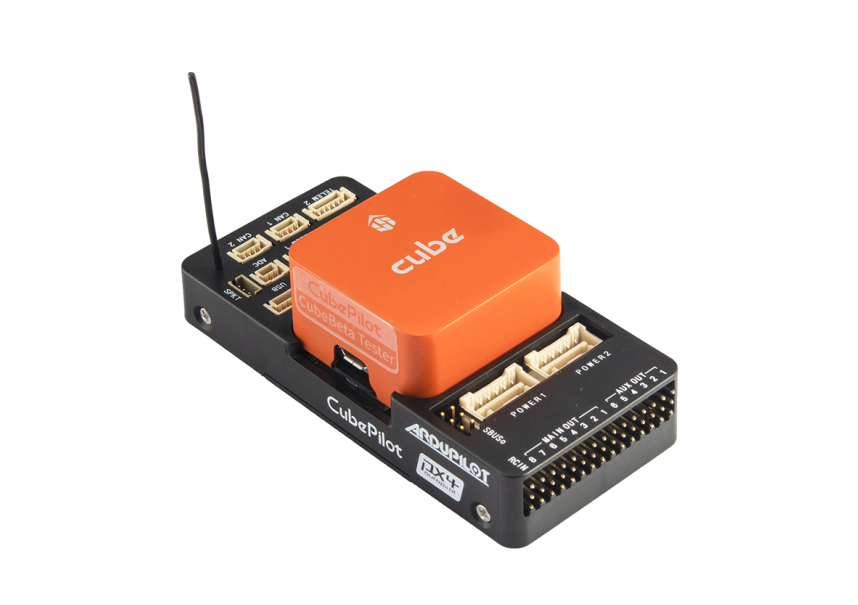
\includegraphics[width=\textwidth]{cube_orange.png}
    \caption{PixHawk CubeOrange飞控\label{fig:cube_orange}}
    \end{minipage}
    \centering
    \begin{minipage}[t]{0.4\textwidth}
    \centering
    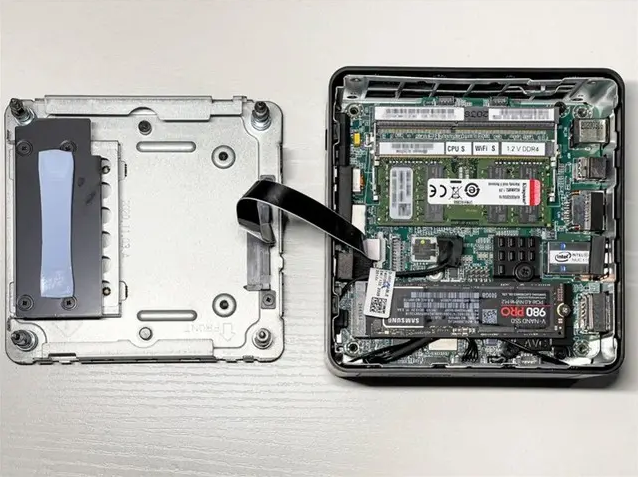
\includegraphics[width=\textwidth]{intel_nuc11_pah_i7.png}
    \caption{Intel NUC11PAHi7迷你电脑\label{fig:nuc}}
    \end{minipage}
\end{figure}

OmniHex暂未部署机载的感知系统,目前使用动作捕捉系统的反馈模拟视觉里程计(visual odometry,VO)的数据。
机载计算机基于VRPN\cite{taylor2001vrpn}与OptiTrack动作捕捉系统进行无线通信,
并将处理后的信号发送给飞控用于位姿估计。

只有上述各个软硬件模块正常工作、协同配合,才能保证飞行器的稳定飞行。
OmniHex的软硬件框架以及模块间的主要数据流向概括为\figref{fig:architecture_1}。
\begin{figure}[ht]
    \centering
    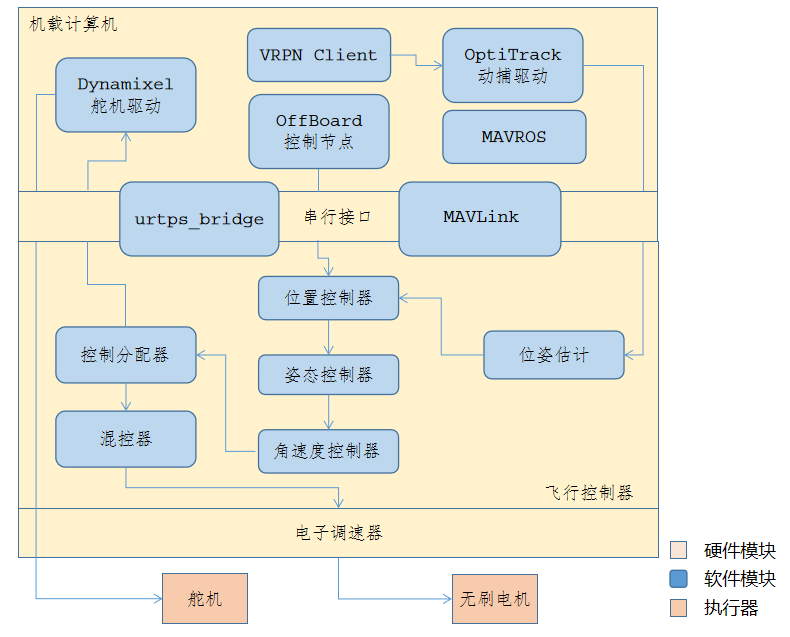
\includegraphics[width = 0.66\textwidth]{architecture_1.png}
    \caption{OmniHex软硬件架构与数据流向简图}
    \label{fig:architecture_1}
\end{figure}

\section{OmniHex的动力学分析}\label{sec:dynamic_analysis}
本节首先建立OmniHex飞行器的动力学模型,
并在动力学模型的基础上分析OmniHex的微分平坦性质,给出平坦输出及相应的微分平坦关系。

为简化模型,且不失模型的实用性,如果不作特别说明,本节及本文后续章节的分析均基于以下假设:
\begin{enumerate}
    \renewcommand{\labelenumi}{(\theenumi)}
    \item 机体结构近似为刚性且对称的,每个旋翼的推力相对质心的力臂长度均为$l$;
    \item 每个旋翼产生的推力和反扭矩正比与其转速的平方,且电机驱动旋翼达到目标转速的调整时间忽略不计;
    \item 各个旋翼所产生的推力和反扭矩相互独立,不考虑空气动力学效应。
    \item 舵机的动态特性与旋翼转速无关;
    \item 机体坐标系$\mathscr{F}_b$的原点$O_b$与飞行器质心重合,且初始时刻机体坐标系轴的指向与世界(惯性)坐标系$\mathscr{F}_W$轴的指向一致;
\end{enumerate}

\subsection{动力学建模与微分平坦性分析}\label{subsec:dynamic_analysis}
\subsubsection{机体坐标系及基本量规定}\label{subsubsec:basic_definition}
在传统欠驱动四旋翼飞行器家族中已经出现了许多种类的结构和形状。从旋翼数量上来看,除了最常见的四旋翼飞行器外,
还出现了三旋翼、六旋翼、八旋翼等飞行器,以及共轴双桨类飞行器;
从机头相对旋翼的位置来看,又可分为X形和十字形等。
大多数多旋翼飞行器的旋翼和结构的布局追求对称性,
且为抵消静止悬停时空气施加的反扭矩,通常相邻和相对的两个旋翼旋转转速相等、方向相反。
\figref{fig:airframe_reference}展示了几种常见构型的多旋翼飞行器及其在PX4开源飞控\footnote{https://github.com/PX4/PX4-Autopilot}中约定的旋翼编号和旋转方向。
\begin{figure}[!ht]
    \setlength{\subfigcapskip}{-1bp}
    \centering
    \begin{minipage}{\textwidth}
    \centering
    \subfigure{\label{fig:quadrotor_x}}\addtocounter{subfigure}{-2}
    \subfigure{\subfigure[X形四旋翼]{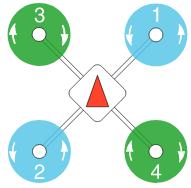
\includegraphics[width=0.2\textwidth]{quadrotor_x.png}}}
    \hspace{0.2em}
    \subfigure{\label{fig:quadrotor_plus}}\addtocounter{subfigure}{-2}
    \subfigure{\subfigure[十字形六旋翼]{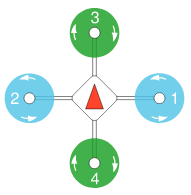
\includegraphics[width=0.2\textwidth]{quadrotor_+.png}}}
    \hspace{0.2em}
    \subfigure{\label{fig:hexarotor_x}}\addtocounter{subfigure}{-2}
    \subfigure{\subfigure[X形四旋翼]{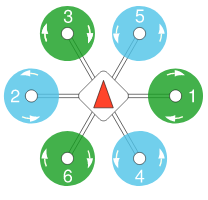
\includegraphics[width=0.2\textwidth]{hexarotor_x.png}}}
    \hspace{0.2em}
    \subfigure{\label{fig:hexarotor_plus}}\addtocounter{subfigure}{-2}
    \subfigure{\subfigure[十字形四旋翼]{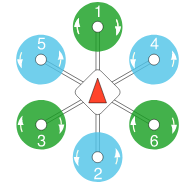
\includegraphics[width=0.2\textwidth]{hexarotor_+.png}}}
    \end{minipage}
    \caption{PX4中几种不同构型的俯视示意图\label{fig:airframe_reference}}
\end{figure}

本课题中OmniHex沿用如\figref{fig:hexarotor_x}所示的X形六旋翼飞行器的旋翼编号和旋转方向。
除此之外,设置机体坐标系$\mathscr{F}_b$为“北-东-地”(NED)坐标系:
机头方向为$x$轴,垂直向机腹为$z$轴,$y$轴指向由右手法则确定;
机臂倾转时的转轴设定为机臂轴线向外,倾转角$\alpha_i$的正方向由右手法则确定。
\figref{fig:basic_definition}对上述规定做出了标注。

\subsubsection{动力学建模}\label{subsubsec:dynamic_modeling}
基于前文所述的假设与规定,可以列写出机体坐标系下OmniHex的刚体动力学Newton-Euler方程:
\begin{align}
    \bm{f}_b &= m(\dot{\bm{v}_b} + \bm{\omega}_b \times \bm{v}_b - \bm{g}_b) \label{equ:newton_equation} \\
    \bm{\tau}_b &= \bm{\omega}_b \times \bm{J}_b\bm{\omega}_b + \bm{J}_b\dot{\bm{\omega}_b} \label{equ:euler_equation}
\end{align}
\begin{tabularx}{\textwidth}{@{}l@{\quad}r@{———}X@{}}
    式中& $m$ &飞行器的总质量;\\
       & $\bm{f}_b$ &旋翼合推力在机体坐标系下的表示;\\
       & $\bm{\tau}_b$ &旋翼合转矩在机体坐标系下的表示;\\
       & $\bm{v}_b$ &飞行器质心速度在机体坐标系下的表示;\\
       & $\bm{\omega}_b$ &飞行器相对世界坐标系的角速度在机体坐标系下的表示;\\
       & $\bm{g}_b$ &重力加速度在机体坐标系下的表示;\\
       & $\bm{J}_b$ &飞行器相对机体坐标系的惯量矩阵;
\end{tabularx}\vspace{3.15bp}
\begin{figure}[!ht]
    \setlength{\subfigcapskip}{-1bp}
    \centering
    \begin{minipage}{\textwidth}
    \centering
    \subfigure{\label{fig:basic_definition_1}}\addtocounter{subfigure}{-2}
    \subfigure{\subfigure[俯视图]{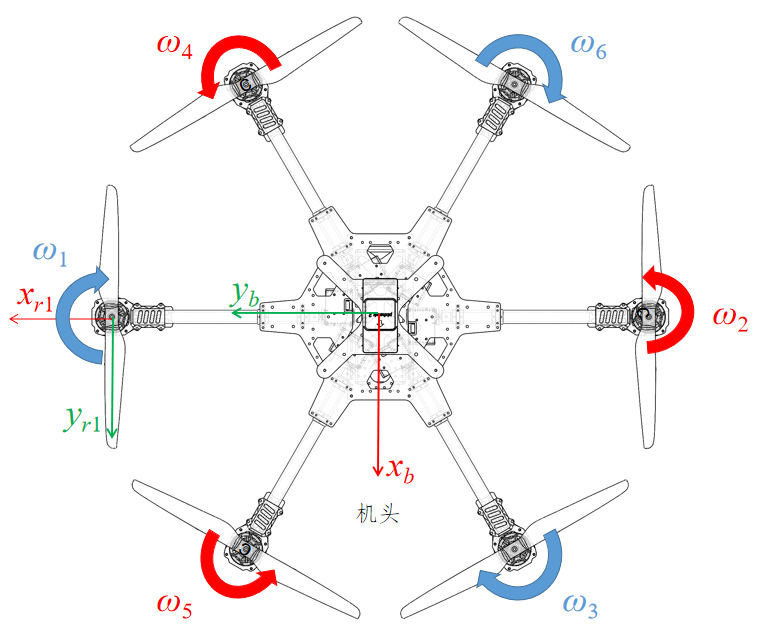
\includegraphics[width=0.4\textwidth]{basic_definition_1.png}}}
    \hspace{0.2em}
    \subfigure{\label{fig:basic_definition_2}}\addtocounter{subfigure}{-2}
    \subfigure{\subfigure[前视图]{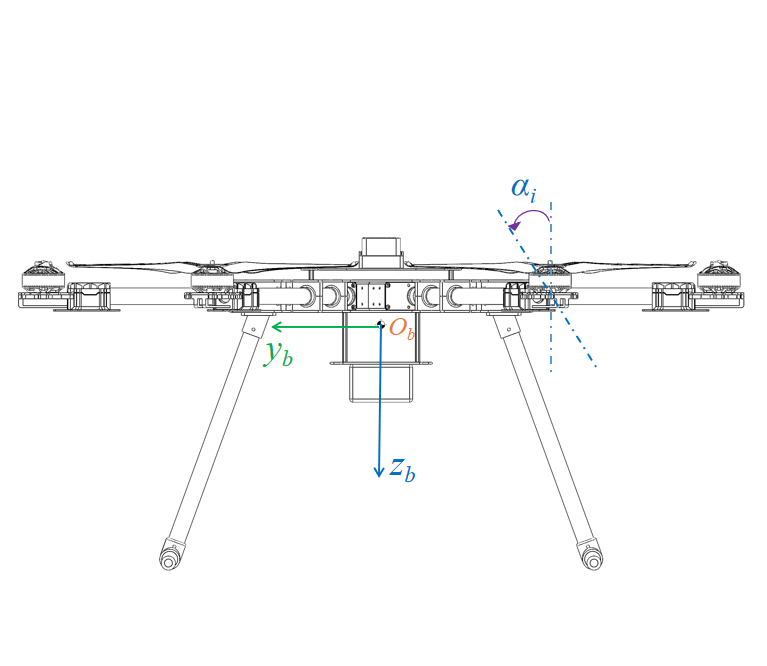
\includegraphics[width=0.4\textwidth]{basic_definition_2.png}}}
    \end{minipage}
    \caption{OmniHex坐标系及相关量规定示意图\label{fig:basic_definition}}
\end{figure}
\equref{equ:newton_equation}及\equref{equ:euler_equation}分别完整描述了OmniHex的平移和旋转动力学特性(实际上可以描述任何刚体),
为后续分析和控制策略的设计提供了依据。

根据先前的假设,每个旋翼所产生的推力和反扭矩与转速的平方成正比,
记旋翼的推力系数为$k_F$、反扭矩系数为$k_M$,则第$i$个旋翼所产生的推力和反扭矩的大小为:
\begin{align}
    f_i &= k_F\omega_i^2 \label{equ:thrust_i}\\
    \tau_i &= k_M\omega_i^2\label{equ:drag_i}
\end{align}

记平方转速向量和机臂倾转角向量为:
\begin{gather}
    \bm{\varOmega} = 
    \begin{bmatrix}
        \varOmega_1 & \cdots & \varOmega_6
    \end{bmatrix}^{\text{T}} = 
    \begin{bmatrix}
        \omega_1^2 & \cdots & \omega_6^2
    \end{bmatrix}^{\text{T}} \in \mathbb{R}^6 \label{equ:square_rotate_speed_vector}\\
    \bm{\alpha} = 
    \begin{bmatrix}
        \alpha_1 & \cdots & \alpha_6
    \end{bmatrix}^{\text{T}} \in \mathbb{R}^6 \label{equ:tilt_angle_vector}
\end{gather}

取OmniHex的控制输入为机体坐标系下的旋翼合推力与和转矩,则平方转速向量与控制输入之间具有如下的映射关系:
\begin{equation}
    \bm{u} = 
    \begin{bmatrix}
        \bm{f}_b^{\text{T}} & \bm{\tau}_b^{\text{T}}
    \end{bmatrix}^{\text{T}} =
    \bm{A}_{\bm{\alpha}}\bm{\varOmega}
    \label{equ:instantaneous_allocation_matrix}
\end{equation}
其中$\bm{A}_{\bm{\alpha}} \in \mathbb{R}^{6\times6}$为分配矩阵,其元素均为$\sin\alpha_i$和$\cos\alpha_i$的线性组合,
由于不考虑倾转舵机的响应时间,又把$\bm{A}_{\bm{\alpha}}$称为瞬时分配矩阵\cite{bodie2018towards}。

给定期望的控制输入$\bm{u}$,要得到对应的执行器指令$\bm{\alpha}$和$\bm{\varOmega}$,需要求解非线性方程组\equref{equ:instantaneous_allocation_matrix}。
一种方法是先确定一组机臂倾转角$\bm{\alpha}$,这样瞬时分配矩阵$\bm{A}_{\bm{\alpha}}$就成为一个已知的非奇异矩阵,进而可解得唯一的转速分配$\bm{\varOmega}$;
不过这种做法存在一个较为严重的问题:一旦$\bm{\alpha}$确定,那么$\bm{\varOmega}$也随之确定,难以选择合适的$\bm{\alpha}$来保证$\varOmega_i$的非负约束。
为避免这个问题,可以对方程组\equref{equ:instantaneous_allocation_matrix}进行变形。首先构造以下中间变量:
\begin{gather}
    \zeta_{ci} = \varOmega_i\cos\alpha_i, \zeta_{si} = \varOmega_i\sin\alpha_i \\
    \bm{\zeta} = 
    \begin{bmatrix}
        \zeta_{c1} & \zeta_{s1} & \cdots & \zeta_{c6} & \zeta_{s6}
    \end{bmatrix}^{\text{T}} \in \mathbb{R}^{12} \label{equ:new_actuator_command_vector}
\end{gather}
则方程组\equref{equ:instantaneous_allocation_matrix}可以变形为如下形式:
\begin{equation}
    \bm{u} = \bm{A}\bm{\zeta} \label{equ:new_allocation_map}
\end{equation}
其中$\bm{A} \in \mathbb{R}^{6\times12}$是常量矩阵,仅与$k_F$、$k_M$和$l$有关,
可以通过其Moore-Penrose伪逆求得中间变量$\bm{\zeta}$:
\begin{equation}
    \bm{\zeta} = \bm{A}^{\dagger}\bm{u} \label{equ:find_zeta}
\end{equation}
然后相应的$\bm{\alpha}$和$\bm{\varOmega}$由下式确定:
\begin{gather}
    \alpha_i = \arctan2(\zeta_{si}, \zeta_{ci}) \label{equ:alpha_i} \\
    \varOmega_i = \sqrt{\zeta_{si}^2 + \zeta_{ci}^2} \label{equ:Omega_i}
\end{gather}

\subsubsection{微分平坦性分析}\label{subsubsec:flatness_analysis}
现代控制理论常常使用如下形式的状态空间方程来对一个非线性动态系统进行描述:
\begin{align}
    &\dot{\bm{x}} = \bm{f}(\bm{x}, \bm{u}), \bm{x} \in \mathbb{R}^n, \bm{u} \in \mathbb{R}^m \label{equ:state_equation} \\
    &\bm{z} = \bm{g}(\bm{x}), \bm{z} \in \mathbb{R}^m \label{equ:output_equation}
\end{align}
在无人机系统中常把状态变量取为位姿与速度的组合:
\begin{equation}
    \begin{aligned}
        \bm{x} &= [p_x,p_y,p_z,\phi,\theta,\psi,v_x,v_y,v_z,\omega_x, \omega_y,\omega_z]^{\text{T}} \\
               &= 
               \begin{bmatrix}
                   \bm{p}^{\text{T}} & \bm{\varepsilon}^{\text{T}} & \bm{v}^{\text{T}} & \bm{\omega}^{\text{T}}
               \end{bmatrix}^{\text{T}} \in \mathbb{R}^{12}
    \end{aligned}
    \label{equ:uav_state}
\end{equation}
即$n=12$。对于欠驱动多旋翼无人机而言,有$m=4$;对于OmniHex这类全驱动多旋翼无人机而言,则有$m=6$。

微分平坦的概念最早由Fliess等人于1995年提出\cite{fliess1995flatness},随后便在机器人轨迹规划领域收到了很大的关注。
利用微分平坦性质可以很方便地从系统的输出$\bm{z}$及其有限阶导数还原出系统的状态变量$\bm{x}$和控制输入$\bm{u}$,
反过来也可以将对系统状态和输入的约束$\mathcal{G}_D(\bm{x}, \bm{u})$转化为对平坦输出及其有限阶导数的约束$\mathcal{G}(\bm{z}, \dot{\bm{z}}, \cdots, \bm{z}^{(s)})$(\figref{fig:constraint_transformation})。
\begin{figure}[ht]
    \centering
    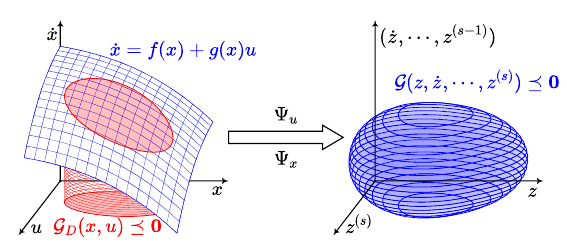
\includegraphics[width = 0.65\textwidth]{constraint_transformation.png}
    \caption{利用微分平坦性质进行约束转化}
    \label{fig:constraint_transformation}
\end{figure}
在平坦输出空间中进行轨迹规划,一来可以对轨迹进行有效降维,使问题得到简化,加快求解速度;
二来能更容易地使轨迹满足机器人的各种约束,更有利于机器人的执行。
欠驱动多旋翼飞行器的微分平坦性质已经被许多人的研究过,Mellinger等人就已经推导出了欠驱动四旋翼飞行器的微分平坦关系\cite{2011minimumsnap},
而全驱动飞行器的微分平坦性质还没有较为成熟的研究。

本课题也将在平坦输出空间中为过驱动飞行器OmniHex进行轨迹规划,
下面将对OmniHex的微分平坦性质进行简要分析。
首先给出微分平坦的定义:
\begin{definition}[(微分平坦)]
    \label{def:differential_flatness}
    考虑\equref{equ:state_equation}所描述的非线性系统,若能够找到一组系统输出$\bm{z} \in \mathbb{R}^m$,
    使得系统状态$\bm{x}$和控制输入$\bm{u}$都能用$\bm{z}$及其有限阶导数表示,即:
    \begin{gather}
        \bm{x} = \bm{\varPsi}_{\bm{x}}(\bm{z}, \dot{\bm{z}}, \cdots, \bm{z}^{(s-1)}) \label{equ:state_flat_map} \\
        \bm{u} =  \bm{\varPsi}_{\bm{u}}(\bm{z}, \dot{\bm{z}}, \cdots, \bm{z}^{(s)}) \label{equ:input_flat_map}
    \end{gather}
    则称该系统为微分平坦系统,相应的输出$\bm{z}$称为平坦输出。
\end{definition}

对于OmniHex这样的全/过驱动飞行器而言,其平坦输出应为一个6维向量。
不妨取系统输出为:
\begin{equation}
    \bm{z} = 
    \begin{bmatrix}
        \bm{p}^{\text{T}} & \bm{\sigma}^{\text{T}}
    \end{bmatrix}^{\text{T}} \in \mathbb{R}^6
    \label{equ:omnihex_output}
\end{equation}
其中$\bm{\sigma} \in \mathbb{R}^3$是机体姿态参数化为3维向量的结果(如欧拉角等),其对应的姿态由一个从$\mathbb{R}^3$到$SO(3)$空间的二阶及以上连续可微满射确定,
若一个姿态对应有多个$\bm{\sigma}$值,则姿态参数化取此满射的一个局部逆映射。
考虑旋转矩阵微分与角速度的关系,有
\begin{equation}
    \bm{\omega}^{\wedge}
     = \dot{\bm{R}}(\bm{\sigma})\bm{R}^{\text{T}}(\bm{\sigma})
     = \sum_{i=1}^3 \frac{\partial \bm{R}(\bm{\sigma})}{\partial \sigma_i}\dot{\sigma}_i\bm{R}^{\text{T}}(\bm{\sigma})
     \label{equ:dsigma_to_omega_hat}
\end{equation}
其中$\sigma_i \in \mathbb{R}^3$表示$\bm{\sigma}$的第$i$个元素;映射$(\cdot)^{\wedge}:\mathbb{R}^3 \mapsto so(3)$表示取向量$\cdot$对应的反对称矩阵(skew-symmetric matrix),
即有关系$\bm{a} \times \bm{b} = \bm{a}^{\wedge}\bm{b}$,
同理可以定义其逆映射$(\cdot)^{\vee}:so(3) \mapsto \mathbb{R}^3$,表示取反对称矩阵对应的向量。
这样机体的角速度$\bm{\omega}$也可以由$\bm{\sigma}$及其导数表示:
\begin{equation}
    \bm{\omega}(\bm{\sigma}, \dot{\bm{\sigma}}) = 
    \left[
        \sum_{i=1}^3 \frac{\partial \bm{R}(\bm{\sigma})}{\partial \sigma_i}\dot{\sigma}_i\bm{R}^{\text{T}}(\bm{\sigma})
    \right]^{\vee}
    \label{equ:dsigma_to_omega}
\end{equation}
进一步可以表示角加速度:
\begin{equation}
    \begin{aligned}
        (\dot{\bm{\omega}})^{\wedge} = \frac{\text{d}\bm{\omega}^{\wedge}}{\text{d}t} &=
        \frac{\text{d}}{\text{d}t}\left(\sum_{i=1}^3 \frac{\partial \bm{R}(\bm{\sigma})}{\partial \sigma_i}\dot{\sigma}_i\bm{R}^{\text{T}}(\bm{\sigma})\right) \\
        &= \sum_{i=1}^3 \left(\sum_{j=1}^3 \frac{\partial^2 \bm{R}}{\partial\sigma_i\partial\sigma_j}\ddot{\sigma}_j\dot{\sigma}_i + \frac{\partial \bm{R}}{\partial \sigma_i}\ddot{\sigma}_i\right)\bm{R}^{\text{T}} + 
        \dot{\bm{R}}\dot{\bm{R}}^{\text{T}}
    \end{aligned}
    \label{equ:dsigma_to_d1omega}
\end{equation}
于是我们得到了状态变量$\bm{x}$关于输出$\bm{z}$及其各阶导数的函数关系:
\begin{equation}
    \bm{x} = 
    \begin{bmatrix}
        \bm{p} \\ \bm{\varepsilon} \\ \bm{v} \\ \bm{\omega}
    \end{bmatrix} = 
    \bm{\varPsi}_{\bm{x}}(\bm{z}, \dot{\bm{z}}) = 
    \begin{bmatrix}
        \bm{p} \\ \bm{\varepsilon}(\bm{\sigma}) \\ \dot{\bm{p}} \\ 
        \left(
        \sum_{i=1}^3 \frac{\partial \bm{R}(\bm{\sigma})}{\partial \sigma_i}\dot{\sigma}_i\bm{R}^{\text{T}}(\bm{\sigma})
        \right)^{\vee}
    \end{bmatrix}
    \label{equ:Psi_x}
\end{equation}
控制输入$\bm{u}$关于输出$\bm{z}$及其各阶导数的函数关系则可根据\equref{equ:newton_equation}和\equref{equ:euler_equation},
结合\equref{equ:dsigma_to_omega}及\equref{equ:dsigma_to_d1omega}确定:
\begin{gather}
    \bm{u} = 
    \begin{bmatrix}
        \bm{f}_b \\ \bm{\tau}_b
    \end{bmatrix} = 
    \bm{\varPsi}_{\bm{u}}(\bm{z}, \dot{\bm{z}}, \ddot{\bm{z}}) = 
    \begin{bmatrix}
        m\bm{R}(\bm{\sigma})(\ddot{\bm{p}} - \bm{g}) \\ 
        \bm{R}(\bm{\sigma})(\bm{\omega} \times \bm{J}(\bm{\sigma})\bm{\omega} + \bm{J}(\bm{\sigma})\dot{\bm{\omega}})
    \end{bmatrix} \label{equ:Psi_u}\\ 
    \bm{J}(\bm{\sigma}) = \bm{R}(\bm{\sigma})\bm{J}_b\bm{R}^{\text{T}}(\bm{\sigma}) \label{sigma_to_J}
\end{gather}

至此我们说明了全驱动多旋翼飞行器是微分平坦系统,\equref{equ:omnihex_output}所选的系统输出$\bm{z}$为平坦输出。
% \section{OmniHex的控制策略}\label{sec:control_policy}


\section{本章小结}\label{sec:summary_2}
本章简要介绍了OmniHex实物系统的设计与搭建,
并基于实际系统建立并分析了OmniHex的动力学模型,
阐明了其是微分平坦系统并给出了平坦输出的形式,
为后续选取平坦输出进行6自由度$SE(3)$轨迹规划提供了依据。

